\begin{figure}[h]
    \centering
    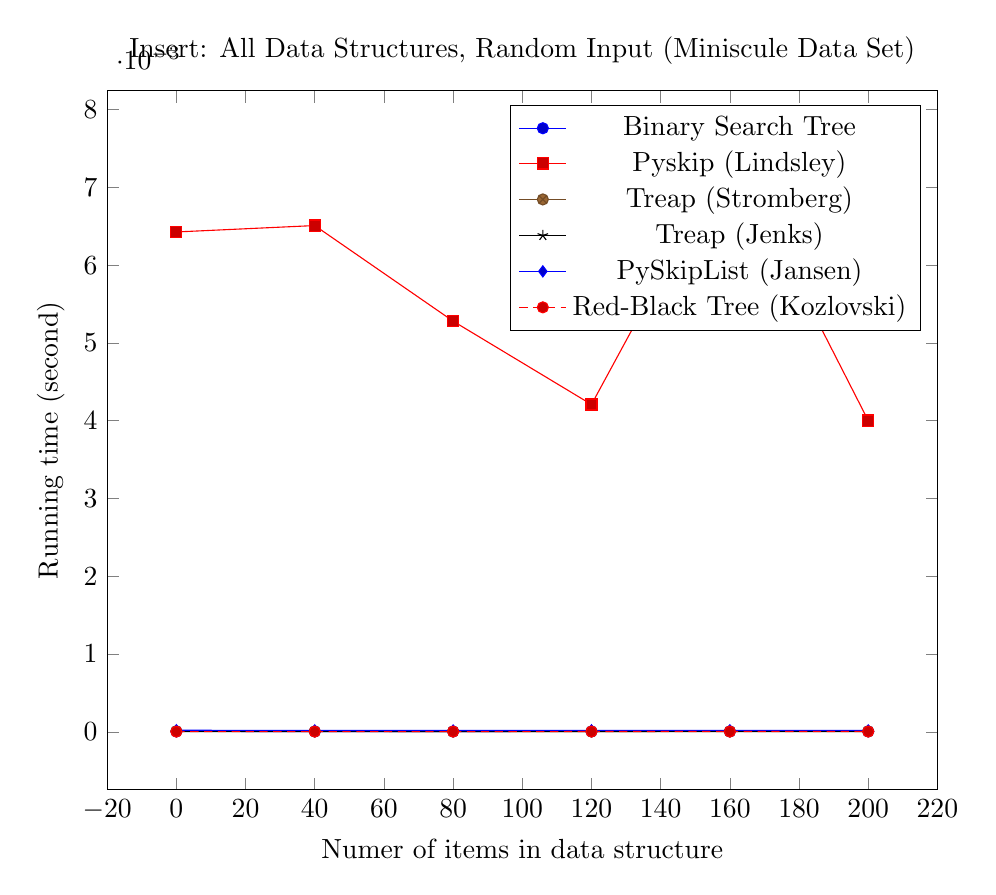
\begin{tikzpicture}
        \begin{axis}[
            xlabel={Numer of items in data structure},
            ylabel={Running time (second)},
            title={Insert: All Data Structures, Random Input (Miniscule Data Set)},
            width=\textwidth
        ]
		\addplot coordinates {
			(0, 4.879040455385564e-06)
			(40, 4.638100185960781e-06)
			(80, 4.427277450247402e-06)
			(120, 5.2404508594783294e-06)
			(160, 4.999510590053547e-06)
			(200, 5.119980724810347e-06)
		};
		\addplot coordinates {
			(0, 0.00642656968820825)
			(40, 0.006508941142809821)
			(80, 0.005279874711059928)
			(120, 0.004208503685633147)
			(160, 0.00749071250555291)
			(200, 0.004001807052020512)
		};
		\addplot coordinates {
			(0, 7.740206154505102e-06)
			(40, 5.300685926812321e-06)
			(80, 4.306807315535011e-06)
			(120, 4.397159916580406e-06)
			(160, 5.180215792099929e-06)
			(200, 6.56562234118141e-06)
		};
		\addplot coordinates {
			(0, 2.710578030740152e-06)
			(40, 2.439520227692782e-06)
			(80, 2.2286974919794033e-06)
			(120, 2.3190500929803904e-06)
			(160, 2.0781098236000163e-06)
			(200, 2.680460497073156e-06)
		};
		\addplot coordinates {
			(0, 2.0028159893969998e-05)
			(40, 1.7799462402035004e-05)
			(80, 1.6805583790757695e-05)
			(120, 1.882345854697931e-05)
			(160, 1.903428128269269e-05)
			(200, 1.7799462402035004e-05)
		};
		\addplot coordinates {
			(0, 2.8310481654525432e-06)
			(40, 2.9816358338319306e-06)
			(80, 3.0719884348329173e-06)
			(120, 3.463516372637088e-06)
			(160, 3.463516372637088e-06)
			(200, 3.463516372637088e-06)
		};
        \legend{Binary Search Tree, Pyskip (Lindsley), Treap (Stromberg), Treap (Jenks), PySkipList (Jansen), Red-Black Tree (Kozlovski)}
        \end{axis}
    \end{tikzpicture}
    \caption{Average of 10 operations, benchmarked every 40, starting at 0.}
\end{figure}